% Graphic for TeX using PGF
% Title: S:\Senior Project\seniorProject2-2020-21-Docs\figs\dia\navigationAlgoFlowchart.dia
% Creator: Dia v0.97.2
% CreationDate: Tue Dec 01 10:48:27 2020
% For: Jason Braker
% \usepackage{tikz}
% The following commands are not supported in PSTricks at present
% We define them conditionally, so when they are implemented,
% this pgf file will use them.
\ifx\du\undefined
  \newlength{\du}
\fi
\setlength{\du}{15\unitlength}
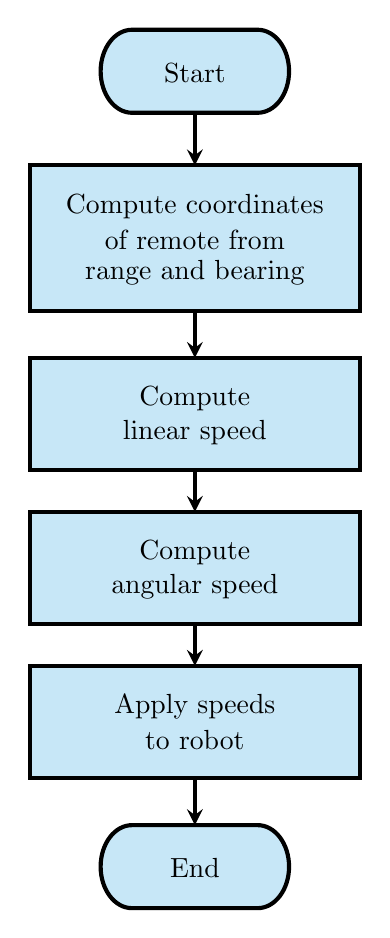
\begin{tikzpicture}
\pgftransformxscale{1.000000}
\pgftransformyscale{-1.000000}
\definecolor{dialinecolor}{rgb}{0.000000, 0.000000, 0.000000}
\pgfsetstrokecolor{dialinecolor}
\definecolor{dialinecolor}{rgb}{1.000000, 1.000000, 1.000000}
\pgfsetfillcolor{dialinecolor}
\pgfsetlinewidth{0.100000\du}
\pgfsetdash{}{0pt}
\pgfsetdash{}{0pt}
\pgfsetbuttcap
\pgfsetmiterjoin
\pgfsetlinewidth{0.100000\du}
\pgfsetbuttcap
\pgfsetmiterjoin
\pgfsetdash{}{0pt}
\definecolor{dialinecolor}{rgb}{0.780392, 0.905882, 0.968627}
\pgfsetfillcolor{dialinecolor}
\pgfpathmoveto{\pgfpoint{19.006275\du}{3.950000\du}}
\pgfpathlineto{\pgfpoint{22.032525\du}{3.950000\du}}
\pgfpathcurveto{\pgfpoint{22.450363\du}{3.950000\du}}{\pgfpoint{22.789088\du}{4.397715\du}}{\pgfpoint{22.789088\du}{4.950000\du}}
\pgfpathcurveto{\pgfpoint{22.789088\du}{5.502285\du}}{\pgfpoint{22.450363\du}{5.950000\du}}{\pgfpoint{22.032525\du}{5.950000\du}}
\pgfpathlineto{\pgfpoint{19.006275\du}{5.950000\du}}
\pgfpathcurveto{\pgfpoint{18.588437\du}{5.950000\du}}{\pgfpoint{18.249713\du}{5.502285\du}}{\pgfpoint{18.249713\du}{4.950000\du}}
\pgfpathcurveto{\pgfpoint{18.249713\du}{4.397715\du}}{\pgfpoint{18.588437\du}{3.950000\du}}{\pgfpoint{19.006275\du}{3.950000\du}}
\pgfusepath{fill}
\definecolor{dialinecolor}{rgb}{0.000000, 0.000000, 0.000000}
\pgfsetstrokecolor{dialinecolor}
\pgfpathmoveto{\pgfpoint{19.006275\du}{3.950000\du}}
\pgfpathlineto{\pgfpoint{22.032525\du}{3.950000\du}}
\pgfpathcurveto{\pgfpoint{22.450363\du}{3.950000\du}}{\pgfpoint{22.789088\du}{4.397715\du}}{\pgfpoint{22.789088\du}{4.950000\du}}
\pgfpathcurveto{\pgfpoint{22.789088\du}{5.502285\du}}{\pgfpoint{22.450363\du}{5.950000\du}}{\pgfpoint{22.032525\du}{5.950000\du}}
\pgfpathlineto{\pgfpoint{19.006275\du}{5.950000\du}}
\pgfpathcurveto{\pgfpoint{18.588437\du}{5.950000\du}}{\pgfpoint{18.249713\du}{5.502285\du}}{\pgfpoint{18.249713\du}{4.950000\du}}
\pgfpathcurveto{\pgfpoint{18.249713\du}{4.397715\du}}{\pgfpoint{18.588437\du}{3.950000\du}}{\pgfpoint{19.006275\du}{3.950000\du}}
\pgfusepath{stroke}
% setfont left to latex
\definecolor{dialinecolor}{rgb}{0.000000, 0.000000, 0.000000}
\pgfsetstrokecolor{dialinecolor}
\node at (20.519400\du,4.990000\du){Start};
\pgfsetlinewidth{0.100000\du}
\pgfsetdash{}{0pt}
\pgfsetdash{}{0pt}
\pgfsetbuttcap
\pgfsetmiterjoin
\pgfsetlinewidth{0.100000\du}
\pgfsetbuttcap
\pgfsetmiterjoin
\pgfsetdash{}{0pt}
\definecolor{dialinecolor}{rgb}{0.780392, 0.905882, 0.968627}
\pgfsetfillcolor{dialinecolor}
\pgfpathmoveto{\pgfpoint{19.006275\du}{23.110600\du}}
\pgfpathlineto{\pgfpoint{22.032525\du}{23.110600\du}}
\pgfpathcurveto{\pgfpoint{22.450363\du}{23.110600\du}}{\pgfpoint{22.789088\du}{23.558315\du}}{\pgfpoint{22.789088\du}{24.110600\du}}
\pgfpathcurveto{\pgfpoint{22.789088\du}{24.662885\du}}{\pgfpoint{22.450363\du}{25.110600\du}}{\pgfpoint{22.032525\du}{25.110600\du}}
\pgfpathlineto{\pgfpoint{19.006275\du}{25.110600\du}}
\pgfpathcurveto{\pgfpoint{18.588437\du}{25.110600\du}}{\pgfpoint{18.249713\du}{24.662885\du}}{\pgfpoint{18.249713\du}{24.110600\du}}
\pgfpathcurveto{\pgfpoint{18.249713\du}{23.558315\du}}{\pgfpoint{18.588437\du}{23.110600\du}}{\pgfpoint{19.006275\du}{23.110600\du}}
\pgfusepath{fill}
\definecolor{dialinecolor}{rgb}{0.000000, 0.000000, 0.000000}
\pgfsetstrokecolor{dialinecolor}
\pgfpathmoveto{\pgfpoint{19.006275\du}{23.110600\du}}
\pgfpathlineto{\pgfpoint{22.032525\du}{23.110600\du}}
\pgfpathcurveto{\pgfpoint{22.450363\du}{23.110600\du}}{\pgfpoint{22.789088\du}{23.558315\du}}{\pgfpoint{22.789088\du}{24.110600\du}}
\pgfpathcurveto{\pgfpoint{22.789088\du}{24.662885\du}}{\pgfpoint{22.450363\du}{25.110600\du}}{\pgfpoint{22.032525\du}{25.110600\du}}
\pgfpathlineto{\pgfpoint{19.006275\du}{25.110600\du}}
\pgfpathcurveto{\pgfpoint{18.588437\du}{25.110600\du}}{\pgfpoint{18.249713\du}{24.662885\du}}{\pgfpoint{18.249713\du}{24.110600\du}}
\pgfpathcurveto{\pgfpoint{18.249713\du}{23.558315\du}}{\pgfpoint{18.588437\du}{23.110600\du}}{\pgfpoint{19.006275\du}{23.110600\du}}
\pgfusepath{stroke}
% setfont left to latex
\definecolor{dialinecolor}{rgb}{0.000000, 0.000000, 0.000000}
\pgfsetstrokecolor{dialinecolor}
\node at (20.519400\du,24.150600\du){End};
\pgfsetlinewidth{0.100000\du}
\pgfsetdash{}{0pt}
\pgfsetdash{}{0pt}
\pgfsetbuttcap
{
\definecolor{dialinecolor}{rgb}{0.000000, 0.000000, 0.000000}
\pgfsetfillcolor{dialinecolor}
% was here!!!
\pgfsetarrowsend{stealth}
\definecolor{dialinecolor}{rgb}{0.000000, 0.000000, 0.000000}
\pgfsetstrokecolor{dialinecolor}
\draw (20.519400\du,5.950000\du)--(20.519400\du,7.217460\du);
}
\definecolor{dialinecolor}{rgb}{0.780392, 0.905882, 0.968627}
\pgfsetfillcolor{dialinecolor}
\fill (16.542550\du,7.217460\du)--(16.542550\du,10.717460\du)--(24.496250\du,10.717460\du)--(24.496250\du,7.217460\du)--cycle;
\pgfsetlinewidth{0.100000\du}
\pgfsetdash{}{0pt}
\pgfsetdash{}{0pt}
\pgfsetmiterjoin
\definecolor{dialinecolor}{rgb}{0.000000, 0.000000, 0.000000}
\pgfsetstrokecolor{dialinecolor}
\draw (16.542550\du,7.217460\du)--(16.542550\du,10.717460\du)--(24.496250\du,10.717460\du)--(24.496250\du,7.217460\du)--cycle;
% setfont left to latex
\definecolor{dialinecolor}{rgb}{0.000000, 0.000000, 0.000000}
\pgfsetstrokecolor{dialinecolor}
\node at (20.519400\du,8.207460\du){Compute coordinates};
% setfont left to latex
\definecolor{dialinecolor}{rgb}{0.000000, 0.000000, 0.000000}
\pgfsetstrokecolor{dialinecolor}
\node at (20.519400\du,9.007460\du){of remote from};
% setfont left to latex
\definecolor{dialinecolor}{rgb}{0.000000, 0.000000, 0.000000}
\pgfsetstrokecolor{dialinecolor}
\node at (20.519400\du,9.807460\du){range and bearing};
\definecolor{dialinecolor}{rgb}{0.780392, 0.905882, 0.968627}
\pgfsetfillcolor{dialinecolor}
\fill (16.542550\du,11.855470\du)--(16.542550\du,14.555470\du)--(24.496250\du,14.555470\du)--(24.496250\du,11.855470\du)--cycle;
\pgfsetlinewidth{0.100000\du}
\pgfsetdash{}{0pt}
\pgfsetdash{}{0pt}
\pgfsetmiterjoin
\definecolor{dialinecolor}{rgb}{0.000000, 0.000000, 0.000000}
\pgfsetstrokecolor{dialinecolor}
\draw (16.542550\du,11.855470\du)--(16.542550\du,14.555470\du)--(24.496250\du,14.555470\du)--(24.496250\du,11.855470\du)--cycle;
% setfont left to latex
\definecolor{dialinecolor}{rgb}{0.000000, 0.000000, 0.000000}
\pgfsetstrokecolor{dialinecolor}
\node at (20.519400\du,12.845470\du){Compute};
% setfont left to latex
\definecolor{dialinecolor}{rgb}{0.000000, 0.000000, 0.000000}
\pgfsetstrokecolor{dialinecolor}
\node at (20.519400\du,13.645470\du){linear speed};
\definecolor{dialinecolor}{rgb}{0.780392, 0.905882, 0.968627}
\pgfsetfillcolor{dialinecolor}
\fill (16.542550\du,15.564030\du)--(16.542550\du,18.264030\du)--(24.496250\du,18.264030\du)--(24.496250\du,15.564030\du)--cycle;
\pgfsetlinewidth{0.100000\du}
\pgfsetdash{}{0pt}
\pgfsetdash{}{0pt}
\pgfsetmiterjoin
\definecolor{dialinecolor}{rgb}{0.000000, 0.000000, 0.000000}
\pgfsetstrokecolor{dialinecolor}
\draw (16.542550\du,15.564030\du)--(16.542550\du,18.264030\du)--(24.496250\du,18.264030\du)--(24.496250\du,15.564030\du)--cycle;
% setfont left to latex
\definecolor{dialinecolor}{rgb}{0.000000, 0.000000, 0.000000}
\pgfsetstrokecolor{dialinecolor}
\node at (20.519400\du,16.554030\du){Compute};
% setfont left to latex
\definecolor{dialinecolor}{rgb}{0.000000, 0.000000, 0.000000}
\pgfsetstrokecolor{dialinecolor}
\node at (20.519400\du,17.354030\du){angular speed};
\definecolor{dialinecolor}{rgb}{0.780392, 0.905882, 0.968627}
\pgfsetfillcolor{dialinecolor}
\fill (16.542550\du,19.272590\du)--(16.542550\du,21.972590\du)--(24.496250\du,21.972590\du)--(24.496250\du,19.272590\du)--cycle;
\pgfsetlinewidth{0.100000\du}
\pgfsetdash{}{0pt}
\pgfsetdash{}{0pt}
\pgfsetmiterjoin
\definecolor{dialinecolor}{rgb}{0.000000, 0.000000, 0.000000}
\pgfsetstrokecolor{dialinecolor}
\draw (16.542550\du,19.272590\du)--(16.542550\du,21.972590\du)--(24.496250\du,21.972590\du)--(24.496250\du,19.272590\du)--cycle;
% setfont left to latex
\definecolor{dialinecolor}{rgb}{0.000000, 0.000000, 0.000000}
\pgfsetstrokecolor{dialinecolor}
\node at (20.519400\du,20.262590\du){Apply speeds};
% setfont left to latex
\definecolor{dialinecolor}{rgb}{0.000000, 0.000000, 0.000000}
\pgfsetstrokecolor{dialinecolor}
\node at (20.519400\du,21.062590\du){to robot};
\pgfsetlinewidth{0.100000\du}
\pgfsetdash{}{0pt}
\pgfsetdash{}{0pt}
\pgfsetbuttcap
{
\definecolor{dialinecolor}{rgb}{0.000000, 0.000000, 0.000000}
\pgfsetfillcolor{dialinecolor}
% was here!!!
\pgfsetarrowsend{stealth}
\definecolor{dialinecolor}{rgb}{0.000000, 0.000000, 0.000000}
\pgfsetstrokecolor{dialinecolor}
\draw (20.519400\du,10.717460\du)--(20.519400\du,11.855470\du);
}
\pgfsetlinewidth{0.100000\du}
\pgfsetdash{}{0pt}
\pgfsetdash{}{0pt}
\pgfsetbuttcap
{
\definecolor{dialinecolor}{rgb}{0.000000, 0.000000, 0.000000}
\pgfsetfillcolor{dialinecolor}
% was here!!!
\pgfsetarrowsend{stealth}
\definecolor{dialinecolor}{rgb}{0.000000, 0.000000, 0.000000}
\pgfsetstrokecolor{dialinecolor}
\draw (20.519400\du,14.555470\du)--(20.519400\du,15.564030\du);
}
\pgfsetlinewidth{0.100000\du}
\pgfsetdash{}{0pt}
\pgfsetdash{}{0pt}
\pgfsetbuttcap
{
\definecolor{dialinecolor}{rgb}{0.000000, 0.000000, 0.000000}
\pgfsetfillcolor{dialinecolor}
% was here!!!
\pgfsetarrowsend{stealth}
\definecolor{dialinecolor}{rgb}{0.000000, 0.000000, 0.000000}
\pgfsetstrokecolor{dialinecolor}
\draw (20.519400\du,18.264030\du)--(20.519400\du,19.272590\du);
}
\pgfsetlinewidth{0.100000\du}
\pgfsetdash{}{0pt}
\pgfsetdash{}{0pt}
\pgfsetbuttcap
{
\definecolor{dialinecolor}{rgb}{0.000000, 0.000000, 0.000000}
\pgfsetfillcolor{dialinecolor}
% was here!!!
\pgfsetarrowsend{stealth}
\definecolor{dialinecolor}{rgb}{0.000000, 0.000000, 0.000000}
\pgfsetstrokecolor{dialinecolor}
\draw (20.519400\du,21.972590\du)--(20.519400\du,23.110600\du);
}
\end{tikzpicture}
